\section{Лекция 6 (23.03)}

\subsection{Метод конечных объёмов}
\subsubsection{Уравнение Пуассона}
Пространственную аппроксимацию дифференицальных операторов
методом конечных объёмов рассмотрим на примере многомерного уравнения Пуассона
\begin{equation}
\label{eq:fvm_pois}
-\nabla^2 u = f,
\end{equation}
которое требуется решить в области $D$. Разобъём эту область
на непересекающиеся подобласти $E_i$, $i = \overline{0, N-1}$ (\figref{fig:fvm_grid}).
Центры ячеек обозначим как $\vec c_i$.

\begin{figure}[h!]
\centering
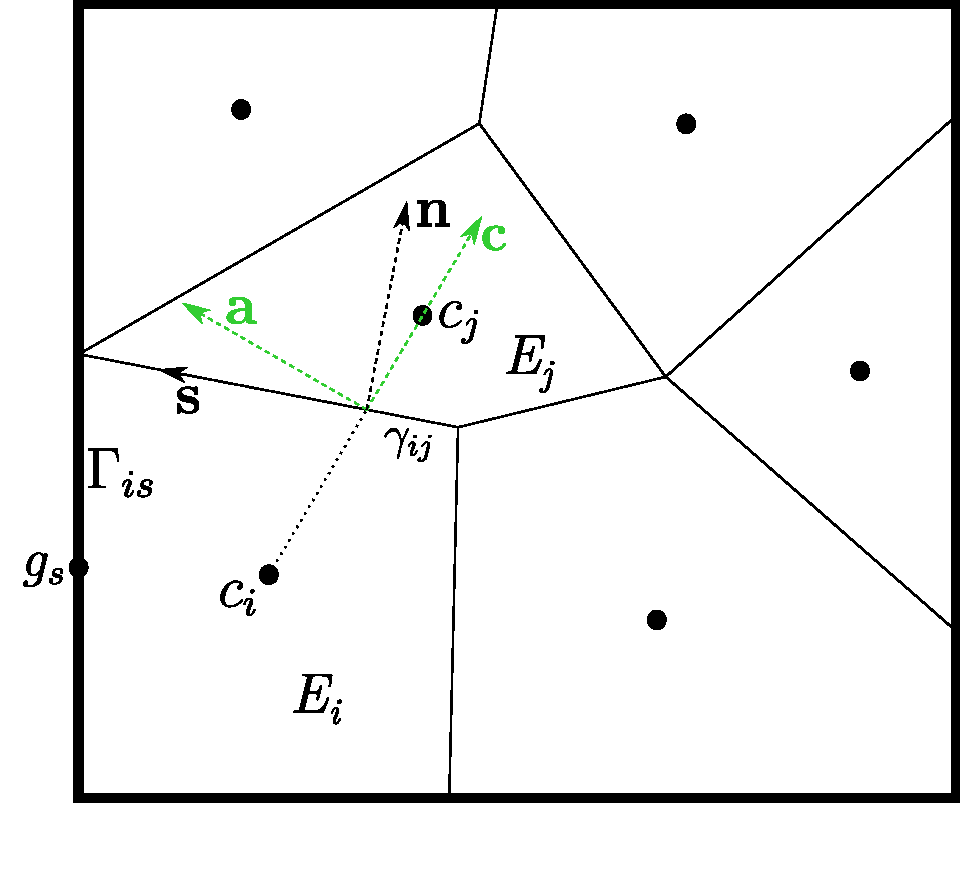
\includegraphics[width=0.4\linewidth]{fvm_grid.pdf}
\caption{Конечнообъёмная сетка}
\label{fig:fvm_grid}
\end{figure}

Проинтегрируем исходное уравнение
по одной из подобластей $E_i$:
\begin{equation*}
-\arint{\nabla^2 u}{E_i}{s} = \arint{f}{E_i}{\vec x}.
\end{equation*}
К интегралу в левой части применим формулу интегрирования по частям \cref{eq:partint_laplace}. Получим
\begin{equation}
\label{eq:fvm_pois_int}
-\arint{\dfr{u}{n}}{\partial E_i}{s} = \arint{f}{E_i}{\vec x}.
\end{equation}
Здесь $\partial E_i$ -- совокупность всех границ подобласти $E_i$,
а $\vec n$ -- внешняя к подобласти нормаль.

Граница ячейки $E_i$ состоит из внутренних граней $\gamma_{ij}$ (индекс $j$ здесь
соответствует индексу соседней ячейки)
и граней $\Gamma_{is}$, лежащих на внешней границе расчётной области $D$.
Тогда интеграл по общей границе ячейки распишется через сумму интегралов по плоским поверхностям
$$
\arint{\dfr{u}{n}}{\partial E_i}{s} = \sum_j\arint{\dfr{u}{n}}{\gamma_{ij}}{s} + \sum_s\arint{\dfr{u}{n}}{\Gamma_{is}}{s}.
$$
Аппроксимирум производную $\dsfr{u}{n}$ на каждой из граней константой.
Тогда её можно вынести из под интегралов и предыдущее выражение записать в виде
\begin{equation}
\label{eq:fvm_gamma_integral}
\arint{\dfr{u}{n}}{\partial E_i}{s} \approx
\sum_j
    \left|
        \gamma_{ij}
    \right|
    \left(
        \dfr{u}{n}
    \right)_{\gamma_{ij}}
+\sum_s
    \left|
        \Gamma_{is}
    \right|
    \left(
        \dfr{u}{n}
    \right)_{\Gamma_{is}}
\end{equation}

Аналогично, анализируя интеграл правой части \cref{eq:fvm_pois_int},
приблизим значение функции правой части $f$ внутри элемента $E_i$ константой $f_i$,
которую отнесём к центру элемента. Тогда
\begin{equation}
\label{eq:fvm_f_integral}
\arint{f}{E_i}{\vec x} \approx f_i \left|E_i\right|.
\end{equation}

Сеточный вектор $\{f_i\}$ -- есть конечнообъёмная аппроксимация
функции $f(\vec x)$ на конечнообъёмную сетку.
Значения $f_i$ при аппроксимации чаще всего находятся как значения в центрах элементов
$$
f_i = f(\vec c_i).
$$
Хотя иногда может быть использовано и другое определение,
следующее из \eqref{eq:fvm_f_integral}:
$$
f_i = \frac{1}{\left| E_i \right|} \arint{f(\vec x)}{E_i}{\vec x}.
$$


\subsubsubsection{Обработка внутренних граней}
Для начала будем рассматривать сетки, в
которых вектора $\vec c$, соединяющие центры ячеек (зедёные вектора на \figref{fig:fvm_grid}),
коллинеарны (или почти коллинеарны) нормалям к граням $\vec n$.
В этом случае производную искомой функции по нормали к грани можно записать в виде
$$
\dfr{u}{n} = \dfr{u}{c}.
$$

Далее определим значения функции $u$ в точках $c_i$, $c_j$ как $u_i$, $u_j$.
Тогда значение производной $\dsfr{u}{n}$ на внутренней грани конечного объёма
может быть приближена конечной разностью
\begin{equation}
\label{eq:fvm_dudn_dudc}
\dfr{u}{n} = \dfr{u}{c} \approx \frac{u_j - u_i}{h_{ij}}, \quad h_{ij} = |\vec c_j - \vec c_i|.
\end{equation}

Определим pebi (perpendicular-bisector) сетки как сетки, удовлетворяющие следующим свойствам
\begin{itemize}
\item линии, соединяющие центры двух соседних ячеек, перпендикулярны грани между этими ячейками;
\item внутренние грани делят линии, соединящие центры соседних ячеек, пополам.
\end{itemize}
Очевидно, что равномерная структурированная сетка удовлетворяет этим свойствам.
Для построения неструктурированных pebi-сеток используют алгоритмы построения ячеек Вороного.
Для pebi-сеток разностная схема \eqref{eq:fvm_dudn_dudc}
является симметричной разностью и, поэтому, имеет второй порядок аппроксимации.

\subsubsubsection{Учёт граничных условий первого рода}
Для вычисления второго слагаемого в правой части 
\cref{eq:fvm_gamma_integral}
следует расписать значение нормальной 
к границе производной вида
$$
\left(\dfr{u}{n}\right)_{\Gamma_{is}}.
$$
Это делается с помощью граничных условий.

Пусть на центре грани $\Gamma_{is}$ задано 
значение искомой функции
\begin{equation}
\label{eq:fvm_bc1}
\vec x \in \Gamma_{is}: \quad u(\vec x) = u^\Gamma.
\end{equation}
Аппроксимацию производных
будем проводить из тех же соображений, которые использовали
при анализе внутренних граней. Только вместо центра соседнего элемента
$c_j$ будем использовать центр грани $g_s$.
В первом приближении, отбрасывая касательные производные, придём к формуле аналогичной \cref{eq:fvm_dudn_dudc}:
\begin{equation}
\label{eq:fvm_bc1_approx}
\dfr{u}{n} \approx \frac{u^\Gamma - u_i}{h_{is}}, \quad h_{is} = \left| \vec g_s  - \vec c_i \right|.
\end{equation}

\subsubsection{Одномерный случай}
Рассмотрим результат конечнообъёмной аппроксимации
задачи \cref{eq:fvm_pois} в одномерном случае
на равномерной сетке с шагом $h$ (\figref{fig:fvm_grid1d}).

\begin{figure}[h!]
\centering
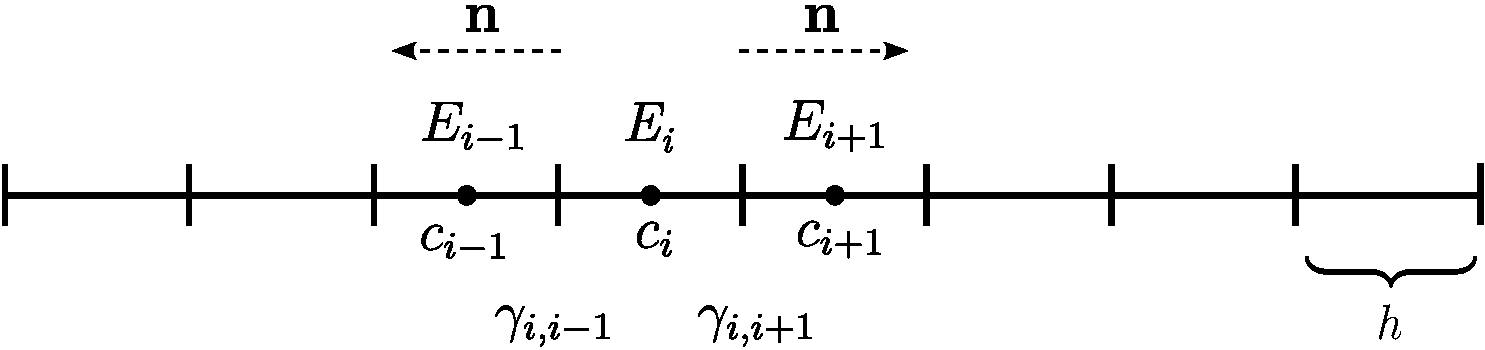
\includegraphics[width=0.6\linewidth]{fvm_grid1d.pdf}
\caption{Одномерная конечнообъёмная сетка}
\label{fig:fvm_grid1d}
\end{figure}

У внутренней ячейки $i$ есть две границы: $\gamma_{i,i-1}$ и $\gamma_{i,i+1}$.
Нормали по этим границам аппроксимируются по формулам \cref{eq:fvm_dudn_approx}:
\begin{align*}
\gamma_{i,i-1}: \quad& \dfr{u}{n} = \frac{u_{i-1}-u_{i}}{h} \\[10pt]
\gamma_{i,i+1}: \quad& \dfr{u}{n} = \frac{u_{i+1}-u_{i}}{h}
\end{align*}
Объём ячейки в одномерном случае равен её длине $h$.
Площадь грани следует положить единице с тем, чтобы
$$
|E_i| = |\gamma| h = h.
$$
Тогда, подставляя эти значения в \cref{eq:fvm_pois_int},
получим знакомую конечноразностную схему аппроксимацию уравнения Пуассона
$$
\frac{-u_{i-1} + 2 u_i - u_{i+1}}{h} = f_i h,
$$
которая имеет второй порядок точности.
Разница с методом конечных разностей здесь состоит в том,
что значения сеточных векторов $\gvec{u}$, $\gvec{f}$ здесь
приписаны к центрам ячеек, а не к их узлам.
Это отличие проявит себя в аппроксимации граничных условий.
Так, если на левой границе задано условие первого рода, то соответствующее уравнение
согласно \cref{eq:fvm_bc1_approx}
примет вид
$$
-\frac{u^\Gamma - u_0}{h/2} - \frac{u_1 - u_0}{h} = f_0 h.
$$
В методе конечных разностей это условие выразилось бы в виде $u_0 = u^\Gamma$.

\subsubsection{Сборка системы линейных уравнений}
Подставим все полученные аппроксимации
\cref{eq:fvm_dudn_dudc,eq:fvm_bc1_approx}
в уравнение \cref{eq:fvm_pois_int}:
\begin{equation*}
-\sum_j
    \frac{|\gamma_{ij}|}{h_{ij}}
         \left(u_j - u_i\right)
-\sum_{s\in{\rm I}}
    \frac{|\Gamma_{is}|}{h_{is}}
        \left(u^\Gamma - u_i\right)
=
f_i |E_i|.
\end{equation*}
Здесь первое слагаемое в левой части отвечает за потоки через внутренние границы,
второе -- граничные условия первого рода.
Далее перенесём все известные значения в правую часть и окончательно
получим линейное уравнение для $i$-го конечного объёма:
\begin{equation}
\label{eq:fvm_slae}
\sum_j
    \frac{|\gamma_{ij}|}{h_{ij}}
         \left(u_i - u_j\right)
+\sum_{s\in{\rm I}}
    \frac{|\Gamma_{is}|}{h_{is}}u_i
 =
f_i |E_i|
+\sum_{s\in{\rm I}}
    \frac{|\Gamma_{is}|}{h_{is}} u^\Gamma
\end{equation}
Таким образом мы получили систему из $N$ (по количеству подобластей) линейных уравнений относительно
неизвестного сеточного вектора $\left\{u_i\right\}$
$$
A u = b.
$$

\subsubsubsection{Алгоритм сборки в цикле по ячейкам}
Матрицу $A$ и правую часть $b$ системы \cref{eq:fvm_slae} можно
собирать в цикле по ячейкам: строчка за строчкой.
Такой алгоритм выглядел бы следующим образом
\begin{equation*}
\begin{array}{ll}
\textbf{for } i = \overline{0, N-1}                          & \textrm{-- цикл по строкам СЛАУ}\\
\qquad b_i = |E_i| f_i                                       & \\
\qquad \textbf{for } j \in \textrm{nei(i)}                   & \textrm{-- цикл по ячейкам, соседним с ячейкой $i$}\\
\qquad \qquad v = \sfrac{|\gamma_{ij}|}{h_{ij}}              & \\
\qquad \qquad A_{ii} \pluseq v                               & \\
\qquad \qquad A_{ij} \minuseq v                              & \\
\qquad \textbf{endfor}                                       & \\
\qquad \textbf{for } s \in \textrm{bnd1(i)}                  & \textrm{-- цикл по граням ячейки $i$ с условиями первого рода}\\
\qquad \qquad v = \sfrac{|\Gamma_{is}|}{h_{is}}              & \\
\qquad \qquad A_{ii} \pluseq v                               & \\
\qquad \qquad b_{i}  \pluseq u^{\Gamma} v                    & \\
\qquad \textbf{endfor}                                       & \\
\textbf{endfor}
\end{array}
\end{equation*}
Первым недостатком такого алгоритма является наличие вложенных циклов.
Во-вторых, коэффициент, отвечающий за поток через внутреннюю грань $\gamma_{ij}$,
равный $\sfrac{|\gamma_{ij}|}{h_{ij}}$ в таком алгоритме будет учитываться дважды:
в строке $i$ и в строке $j$.

\subsubsubsection{Алгоритм сборки в цикле по граням}
Вместо общего цикла по ячейкам, будем использовать цикл по граням.
В таком цикле коэффициенты потоков будут вычисляться один раз
и вставляться сразу в две строки матрицы, соответствующие соседним с гранью ячейкам.
Вложенных циклов в такой постановке удаётся избежать, потому
что у грани есть только две соседние ячейки (в то время как у ячейки может быть произвольное
количество соседних граней).

Разделим все грани на исходной сетки на внутренние и граничные (отдельный набор для каждого вида граничных условий).
Тогда для внутренних граней можно записать
\begin{equation}
\label{eq:fvm_assem_internal}
\begin{array}{ll}
\textbf{for } s \in\textrm{internal}                     & \textrm{-- цикл по внутренним граням}\\ 
\qquad i,j = \textrm{nei\_cells(s)}                      & \textrm{-- две ячейки, соседние с текущей гранью}\\
\qquad v = \sfrac{|\gamma_{ij}|}{h_{ij}}                 & \\
\qquad A_{ii} \pluseq  v; \quad A_{jj} \pluseq  v        & \textrm{-- диагональные коэффициенты матрицы}\\ 
\qquad A_{ij} \minuseq v; \quad A_{ji} \minuseq v        & \textrm{-- внедиагональные коэффициенты матрицы}\\
\textbf{endfor}                                          & \\
\end{array}
\end{equation}
Граничные условия учитываются в отдельных циклах.
Здесь будем учитывать, что у грани, принадлежащей
границе области, есть только одна соседняя ячейка.
Условия первого рода:
\begin{equation}
\label{eq:fvm_assem_bc1}
\begin{array}{ll}
\textbf{for } s \in\textrm{bnd1}                         & \textrm{-- грани с условиями первого рода}\\ 
\qquad i = \textrm{nei\_cells(s)}                        & \textrm{-- соседняя с граничной гранью ячейка}\\
\qquad v = \sfrac{|\Gamma_{is}|}{h_{is}}                 & \\
\qquad A_{ii} \pluseq  v                                 & \\ 
\qquad b_{i} \pluseq u^\Gamma v                          & \\
\textbf{endfor}                                          & \\
\end{array}
\end{equation}
Первое слагаемое в правой части
\cref{eq:fvm_slae}
учтём отдельным циклом:
\begin{equation}
\label{eq:fvm_assem_f}
\begin{array}{ll}                                         & \\
\textbf{for } i = \overline{0,N-1}                        & \textrm{-- цикл по ячейкам}\\ 
\qquad b_i = |E_i| f_i                                    & \\
\textbf{endfor}                                           &
\end{array}
\end{equation}

\subsection{Задание для самостоятельной работы}
\label{sec:hw_fvm2d}) 
В тесте \cvar{poisson1-fvm} из файла \ename{poisson_fvm_solve_test.cpp}
реализовано решение одномерного уравнения Пуассона с граничными условиями первого рода.
Проводится расчёт на сгущающихся сетках с количеством ячеек от 10 до 1000
и расчитываются среднеквадратичные нормы отклонения полученного численного решения от точного.
Решения сохраняются в vtk-файлы \ename{poisson1_fvm_n={}.vtk}.



Отталкиваясь от этой реализации необходимо:
\begin{enumerate}
\item написать аналогичный тест для двумерного уравнения и случая неструктурированных сеток,
\item провести серию расчётов на сгущающихся сетках разных типов (структурированных, pebi и скошенных)
\item визуализировать решение, полученное на этих сетках
\item построить графики сходимости решения и определить порядок аппроксимации метода
\end{enumerate}

\paragraph{Построение неструктурированных сеток}
В папке \ename{test_data} корневой директории репозитория
лежат скрипты построения сеток в программе \ename{HybMesh}:
\begin{itemize}
\item \ename{pebigrid.py} -- pebi--сетка,
\item \ename{tetragrid.py} -- сетка, состоящая из произвольных (скошенных) трех- и четырехугольников.
\end{itemize}
Инструкции по запуску этих скриптов смотри п. \ref{sec:hybmesh}.
Эти скрипты строят равномерную неструктурированную сетку
в единичном квадрате
и записывают её в файл vtk, который впоследствии можно загрузить
в расчётную программу.
В каждом из скриптов есть параметр \cvar{N}, означающий
примерное количество ячеек в итоговой сетке.
Меняя его значение можно строить сетки разного разрешения.

Для загрузки построенной сетки в решатель необходимо файл
с сеткой поместить в каталог \ename{test_data}
и далее загрузить её в класс \cvar{UnstructuredGrid2D}.
Нижеследующий код прочитает файл \ename{test_data/pebigrid.vtk}
и создаст рабочий класс с использованием прочитанной сетки
\begin{cppcode}
std::string fn = test_directory_file("pebigrid.vtk");
UnstructuredGrid2D grid = UnstructuredGrid2D::vtk_read(fn);
\end{cppcode}

\paragraph{Рекомендации к программированию}
При написании новых тестов следует переиспользовать уже написанный код, избегая копирования.
Для этого необходимо пользоваться механизмами наследования классов.
В частности, следует обратить внимание, что все сетки наследуются
от единого интерфейса \cvar{IGrid}. А уже написанный ``одномерный'' код 
в своей алгоритмической части использует только функции этого интерфейса.
